\titre{}
\theme{derivation}
\auteur{Nathan Scheinmann}
\niveau{3M}
\source{sesamath3e}
\type{serie}
\piments{2}
\pts{}
\annee{2425}

\contenu{
\tcblower
On dispose de 288 mètres de clôture grillagée pour construire 6 enclos pour un zoo le plan ci-contre :

\begin{center}
	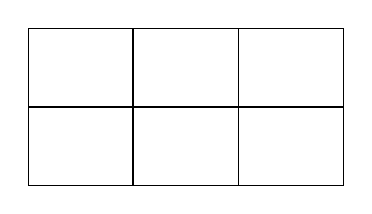
\begin{tikzpicture}
\draw (0,0) rectangle (4,2);
\draw (1.33,0) -- (1.33,2);
\draw (2.67,0) -- (2.67,2);
\draw (0,1) -- (4,1);
\end{tikzpicture}
\end{center}

Quelles dimensions donner à ces enclos de manière à maximiser leur surface au sol ?
}
\correction{

}

